\documentclass[tikz, border=50pt]{standalone}

\usepackage{tikz}
\usepackage{medl_colors}
\usepackage{amsmath,xstring}
\usepackage{ifthen}
\usepackage{moresize}
\usetikzlibrary{shapes.multipart, shapes.geometric, arrows.meta}
\usetikzlibrary{matrix, calc, positioning,fit, backgrounds}
\begin {document}

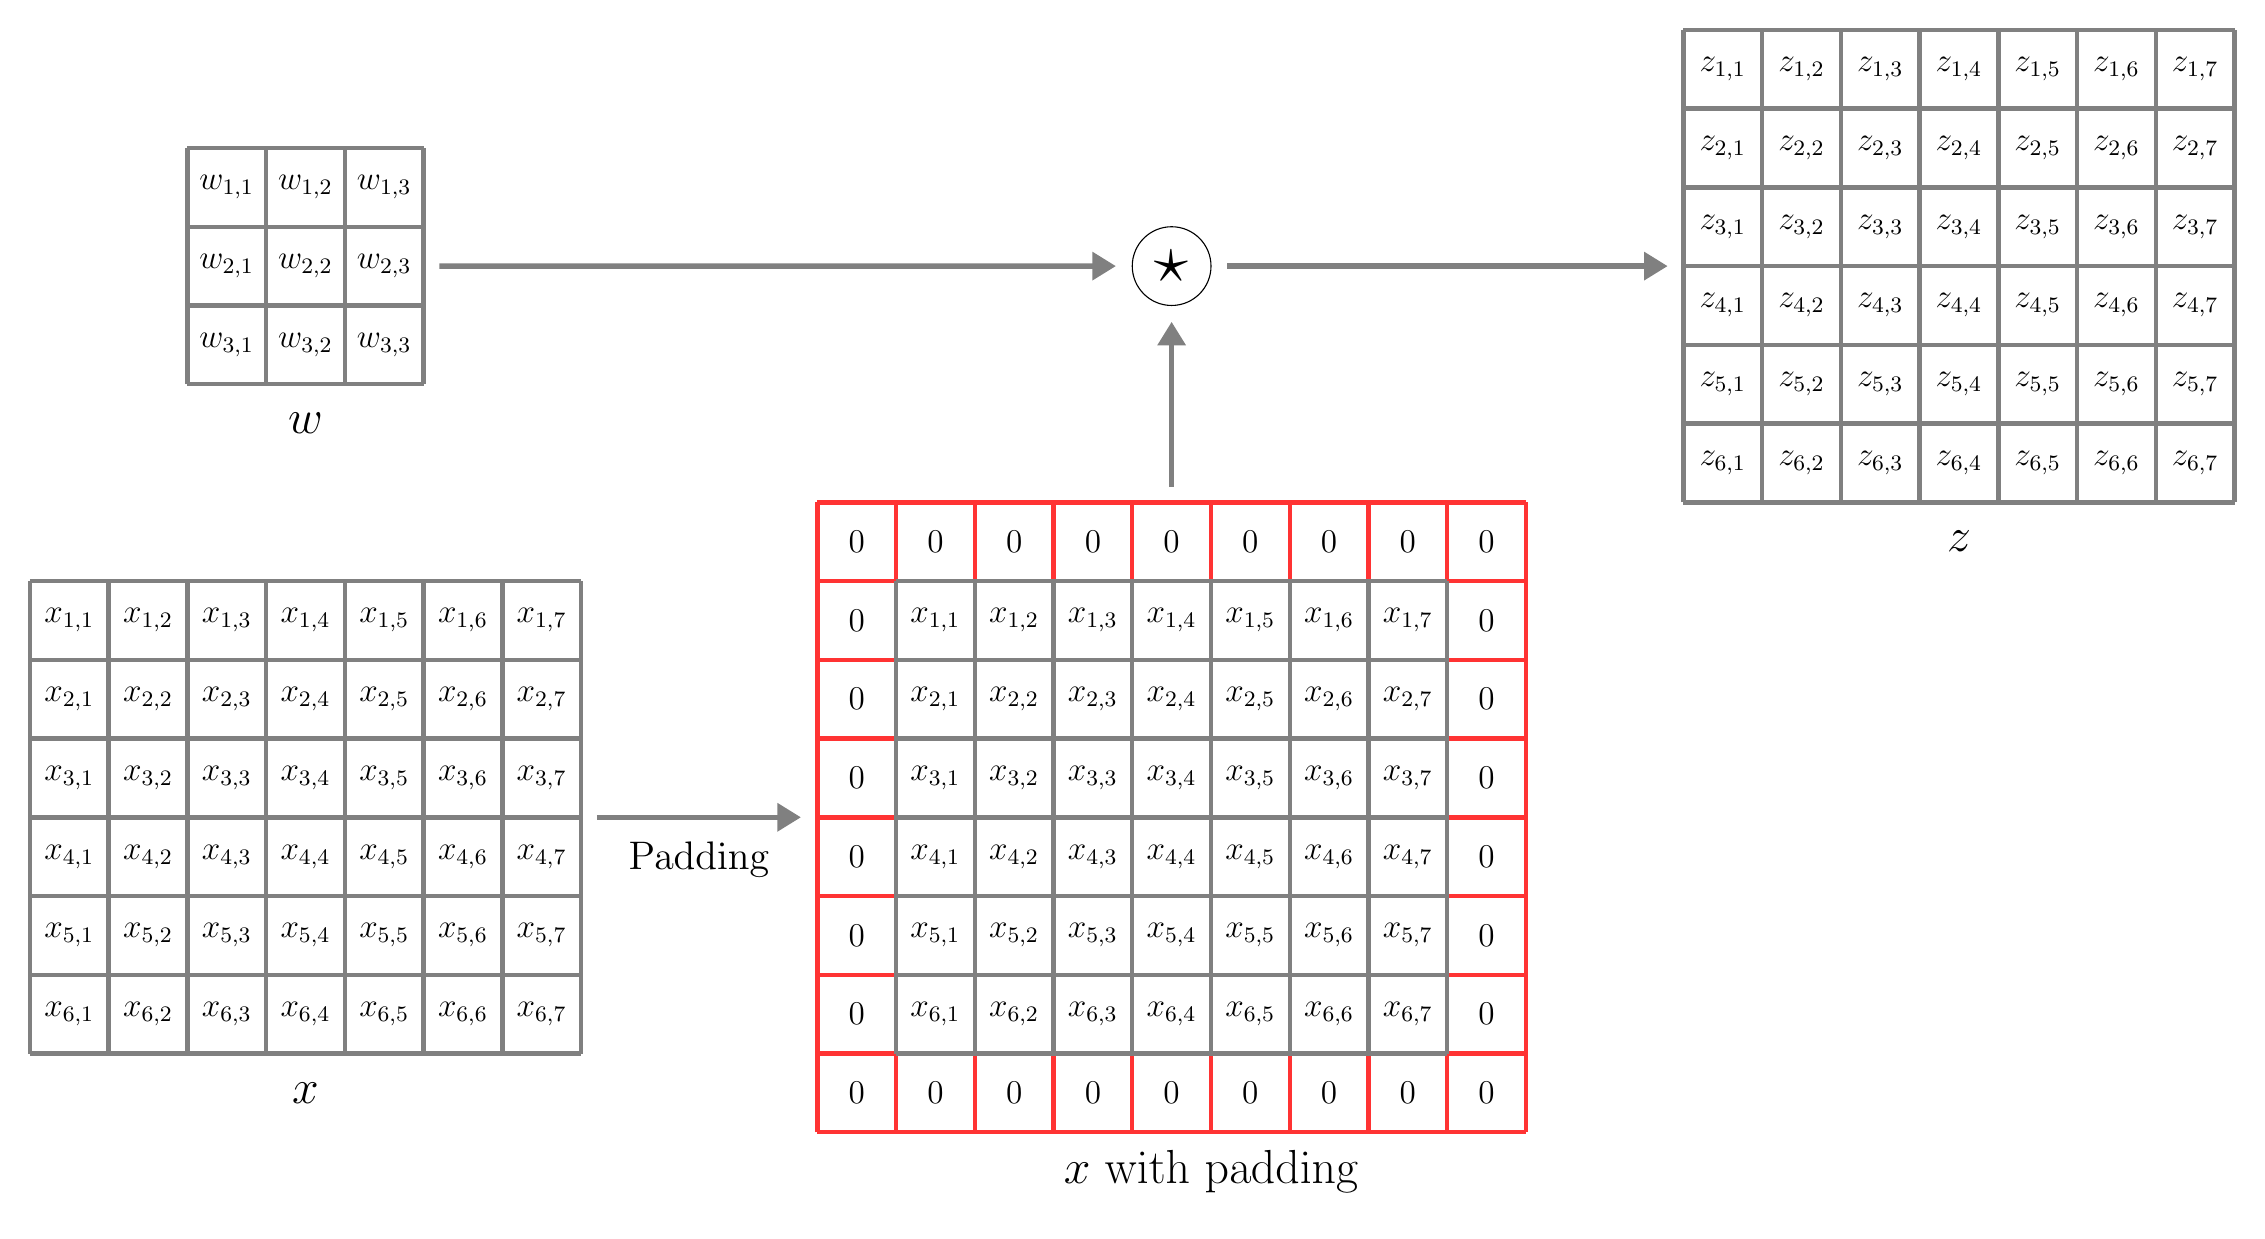
\begin{tikzpicture}[every node/.style={minimum size=1cm},on grid]

\begin{scope}%[every node/.append style={yslant=0.3},yslant=0.3]

\newcommand\slantarray[7]{
    \foreach \i in {1,...,#3}{
        \foreach \j in {1,...,#4}{
            \IfEq{#5}{0}
            {
                \ifthenelse{\j=#4 \OR \i=#3 \OR \j=1 \OR \i=1 }
                {
                    \node (node-#7\i\j) at (#1+\i-.5, #2-\j+.5) {\large $#5$};       
                }
                {
                }
            }
            {
                \node (node-#7\i\j) at (#1+\i-.5, #2-\j+.5) {\large $#5_{\j,\i}$};
            }
            
        }
    }
    \draw[#6, ultra thick] (#1,#2) grid[step=1] (#1+#3, #2-#4) ;
}

    \begin{scope}[yshift=.5cm]
        \slantarray{2}{2}{3}{3}{w}{black!50}{1};
    \end{scope}
    \slantarray{0}{-3}{7}{6}{x}{black!50}{2};
    \slantarray{10}{-2}{9}{8}{0}{red!80}{3};
    \slantarray{11}{-3}{7}{6}{x}{black!50}{4};
    \slantarray{21}{4}{7}{6}{z}{black!50}{5};

\node at (3.5,-1) {\LARGE $w$};
\node at (3.5,-9.5) {\LARGE $x$};
\node at (15,-10.5) {\LARGE $x$ with   padding};
\node at (24.5,-2.5) {\LARGE $z$};
\node [draw, circle] at (14.5,1) (circle) {\Huge $\star$};

\draw[-Triangle, draw=black!50, line width=.7mm] (node-273)+(7mm,-5mm) -- ([xshift=-2mm, yshift=-5mm]node-314.west) node[pos=.5, below] {\Large Padding};
\draw[-Triangle, draw=black!50, line width=.7mm] (node-132)+(7mm,0mm) -- ([xshift=-2mm]circle.west) {};
\draw[Triangle-, draw=black!50, line width=.7mm] (node-513)+(-7mm,-5mm) -- ([xshift=2mm]circle.east) {};
\draw[-Triangle, draw=black!50, thick, line width=.7mm] (node-351)+(0mm, 7mm) -- ([yshift=-2mm]circle.south) {};

\end{scope}
\end{tikzpicture}
\end{document}